\documentclass[8pt,aspectratio=169]{beamer}
\usetheme{Madrid}
\usepackage{graphicx}
\usepackage{booktabs}
\usepackage{adjustbox}
\usepackage{multicol}
\usepackage{amsmath}
\usepackage{amssymb}
\usepackage{listings}
\usepackage{xcolor}

% Color definitions
\definecolor{mlblue}{RGB}{0,102,204}
\definecolor{mlpurple}{RGB}{51,51,178}
\definecolor{mllavender}{RGB}{173,173,224}
\definecolor{mllavender2}{RGB}{193,193,232}
\definecolor{mllavender3}{RGB}{204,204,235}
\definecolor{mllavender4}{RGB}{214,214,239}
\definecolor{mlorange}{RGB}{255, 127, 14}
\definecolor{mlgreen}{RGB}{44, 160, 44}
\definecolor{mlred}{RGB}{214, 39, 40}
\definecolor{mlgray}{RGB}{127, 127, 127}

% Additional colors for template compatibility
\definecolor{lightgray}{RGB}{240, 240, 240}
\definecolor{midgray}{RGB}{180, 180, 180}

% Apply custom colors to Madrid theme
\setbeamercolor{palette primary}{bg=mllavender3,fg=mlpurple}
\setbeamercolor{palette secondary}{bg=mllavender2,fg=mlpurple}
\setbeamercolor{palette tertiary}{bg=mllavender,fg=white}
\setbeamercolor{palette quaternary}{bg=mlpurple,fg=white}
\setbeamercolor{structure}{fg=mlpurple}
\setbeamercolor{section in toc}{fg=mlpurple}
\setbeamercolor{subsection in toc}{fg=mlblue}
\setbeamercolor{title}{fg=mlpurple}
\setbeamercolor{frametitle}{fg=mlpurple,bg=mllavender3}
\setbeamercolor{block title}{bg=mllavender2,fg=mlpurple}
\setbeamercolor{block body}{bg=mllavender4,fg=black}

\setbeamertemplate{navigation symbols}{}
\setbeamertemplate{itemize items}[circle]
\setbeamertemplate{enumerate items}[default]
\setbeamersize{text margin left=5mm,text margin right=5mm}

\newcommand{\bottomnote}[1]{%
\vfill
\vspace{-2mm}
\textcolor{mllavender2}{\rule{\textwidth}{0.4pt}}
\vspace{1mm}
\footnotesize
\textbf{#1}
}

% TikZ and pgfplots packages
\usepackage{tikz}
\usepackage{pgfplots}
\pgfplotsset{compat=1.18}
\usetikzlibrary{arrows.meta, positioning, shapes.geometric, shapes.symbols, calc, decorations.pathmorphing, mindmap}

\title{Tokenomics \& Mechanism Design: A Visual Introduction}
\subtitle{Standalone Mini-Lecture}
\author{Prof.~Dr.~Joerg Osterrieder}
\institute{University Lecture Series}
\date{\today}
\begin{document}

% Frame 1: Title
\begin{frame}[plain]
\vspace{2cm}
\begin{center}
{\Huge\color{mlpurple} Tokenomics \& Mechanism Design: A Visual Introduction}\\[0.4cm]
{\Large\color{mlblue} Standalone Mini-Lecture}\\[0.3cm]
\textcolor{mlgray}{\rule{6cm}{0.4pt}}\\[0.3cm]
{\small\itshape ``Tokenomics is where economics meets cryptography -- design the incentives, and the system runs itself'' -- Vitalik Buterin}\\[1.5cm]
{\normalsize Prof.~Dr.~Joerg Osterrieder}\\[0.2cm]
{\small University Lecture Series}\\[0.2cm]
{\small \today}
\end{center}

\bottomnote{This mini-lecture covers tokenomics fundamentals: supply models, utility types, bonding curves, incentive design, token distribution, vesting schedules, and real-world case studies.}
\end{frame}

% Frame 2: What is Tokenomics?
\begin{frame}{What is Tokenomics?}
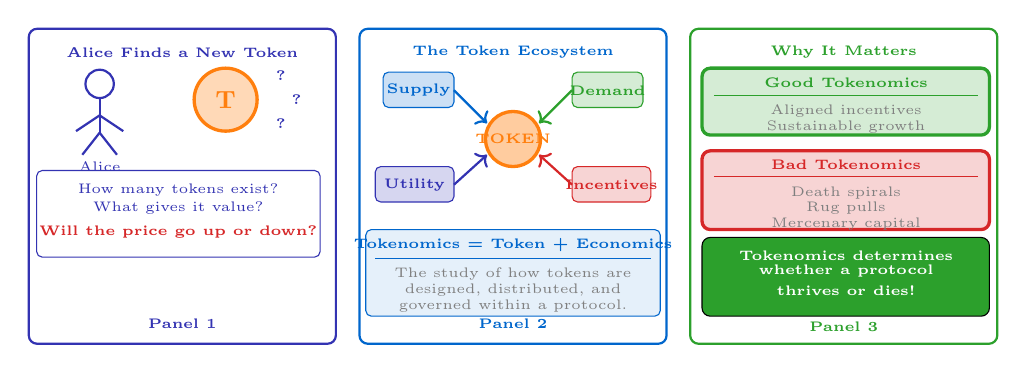
\begin{tikzpicture}
  % Panel borders
  \draw[thick, mlpurple, rounded corners=3pt] (0.1,0.2) rectangle (4.0,4.2);
  \draw[thick, mlblue,   rounded corners=3pt] (4.3,0.2) rectangle (8.2,4.2);
  \draw[thick, mlgreen,  rounded corners=3pt] (8.5,0.2) rectangle (12.4,4.2);

  % --- Panel 1: Alice discovers a token ---
  \node[font=\tiny\bfseries, mlpurple] at (2.05,3.9) {Alice Finds a New Token};
  % Alice stick figure
  \draw[mlpurple,thick] (1.0,3.5) circle (0.18);
  \draw[mlpurple,thick] (1.0,3.32) -- (1.0,2.88);
  \draw[mlpurple,thick] (1.0,3.1) -- (0.7,2.9);
  \draw[mlpurple,thick] (1.0,3.1) -- (1.3,2.9);
  \draw[mlpurple,thick] (1.0,2.88) -- (0.78,2.60);
  \draw[mlpurple,thick] (1.0,2.88) -- (1.22,2.60);
  \node[font=\tiny, mlpurple] at (1.0,2.45) {Alice};
  % Token icon
  \draw[fill=mlorange!30, draw=mlorange, very thick] (2.6,3.3) circle (0.4);
  \node[font=\small\bfseries, mlorange] at (2.6,3.3) {T};
  % Question marks
  \node[font=\tiny\bfseries, mlpurple] at (3.3,3.6) {?};
  \node[font=\tiny\bfseries, mlpurple] at (3.5,3.3) {?};
  \node[font=\tiny\bfseries, mlpurple] at (3.3,3.0) {?};
  % Speech bubble
  \draw[fill=white, draw=mlpurple, rounded corners=2pt] (0.2,1.3) rectangle (3.8,2.4);
  \node[font=\tiny, mlpurple, align=center] at (2.0,2.15) {How many tokens exist?};
  \node[font=\tiny, mlpurple, align=center] at (2.0,1.92) {What gives it value?};
  \node[font=\tiny\bfseries, mlred, align=center] at (2.0,1.62) {Will the price go up or down?};
  \node[font=\tiny\bfseries, mlpurple] at (2.05,0.45) {Panel 1};

  % --- Panel 2: The Token Ecosystem ---
  \node[font=\tiny\bfseries, mlblue] at (6.25,3.9) {The Token Ecosystem};
  % Central token
  \draw[fill=mlorange!40, draw=mlorange, very thick] (6.25,2.8) circle (0.35);
  \node[font=\tiny\bfseries, mlorange] at (6.25,2.8) {TOKEN};
  % Surrounding elements
  \draw[fill=mlblue!20, draw=mlblue, rounded corners=2pt] (4.6,3.2) rectangle (5.5,3.65);
  \node[font=\tiny\bfseries, mlblue, align=center] at (5.05,3.42) {Supply};
  \draw[->, thick, mlblue] (5.5,3.42) -- (5.92,3.0);
  \draw[fill=mlgreen!20, draw=mlgreen, rounded corners=2pt] (7.0,3.2) rectangle (7.9,3.65);
  \node[font=\tiny\bfseries, mlgreen, align=center] at (7.45,3.42) {Demand};
  \draw[->, thick, mlgreen] (7.0,3.42) -- (6.58,3.0);
  \draw[fill=mlpurple!20, draw=mlpurple, rounded corners=2pt] (4.5,2.0) rectangle (5.5,2.45);
  \node[font=\tiny\bfseries, mlpurple, align=center] at (5.0,2.22) {Utility};
  \draw[->, thick, mlpurple] (5.5,2.22) -- (5.92,2.6);
  \draw[fill=mlred!20, draw=mlred, rounded corners=2pt] (7.0,2.0) rectangle (8.0,2.45);
  \node[font=\tiny\bfseries, mlred, align=center] at (7.5,2.22) {Incentives};
  \draw[->, thick, mlred] (7.0,2.22) -- (6.58,2.6);
  % Bottom definition
  \draw[fill=mlblue!10, draw=mlblue, rounded corners=2pt] (4.38,0.55) rectangle (8.12,1.65);
  \node[font=\tiny\bfseries, mlblue, align=center] at (6.25,1.45) {Tokenomics = Token + Economics};
  \draw[mlblue, thin] (4.5,1.28) -- (8.0,1.28);
  \node[font=\tiny, mlgray, align=center] at (6.25,1.08) {The study of how tokens are};
  \node[font=\tiny, mlgray, align=center] at (6.25,0.88) {designed, distributed, and};
  \node[font=\tiny, mlgray, align=center] at (6.25,0.68) {governed within a protocol.};
  \node[font=\tiny\bfseries, mlblue] at (6.25,0.45) {Panel 2};

  % --- Panel 3: Why It Matters ---
  \node[font=\tiny\bfseries, mlgreen] at (10.45,3.9) {Why It Matters};
  % Good tokenomics box
  \draw[fill=mlgreen!20, draw=mlgreen, very thick, rounded corners=3pt] (8.65,2.85) rectangle (12.3,3.7);
  \node[font=\tiny\bfseries, mlgreen, align=center] at (10.48,3.52) {Good Tokenomics};
  \draw[mlgreen, thin] (8.8,3.35) -- (12.15,3.35);
  \node[font=\tiny, mlgray, align=center] at (10.48,3.15) {Aligned incentives};
  \node[font=\tiny, mlgray, align=center] at (10.48,2.95) {Sustainable growth};
  % Bad tokenomics box
  \draw[fill=mlred!20, draw=mlred, very thick, rounded corners=3pt] (8.65,1.65) rectangle (12.3,2.65);
  \node[font=\tiny\bfseries, mlred, align=center] at (10.48,2.48) {Bad Tokenomics};
  \draw[mlred, thin] (8.8,2.32) -- (12.15,2.32);
  \node[font=\tiny, mlgray, align=center] at (10.48,2.12) {Death spirals};
  \node[font=\tiny, mlgray, align=center] at (10.48,1.92) {Rug pulls};
  \node[font=\tiny, mlgray, align=center] at (10.48,1.72) {Mercenary capital};
  % Key point
  \draw[fill=mlgreen, rounded corners=3pt] (8.65,0.55) rectangle (12.3,1.55);
  \node[font=\tiny\bfseries, white, align=center] at (10.48,1.32) {Tokenomics determines};
  \node[font=\tiny\bfseries, white, align=center] at (10.48,1.12) {whether a protocol};
  \node[font=\tiny\bfseries, white, align=center] at (10.48,0.88) {thrives or dies!};
  \node[font=\tiny\bfseries, mlgreen] at (10.45,0.42) {Panel 3};
\end{tikzpicture}

\bottomnote{Tokenomics is the economic design of a crypto token: its supply, demand, utility, and incentive structures. Good tokenomics aligns participant behavior; bad tokenomics leads to death spirals and value collapse.}
\end{frame}

% Frame 3: Supply Models
\begin{frame}{Token Supply Models}
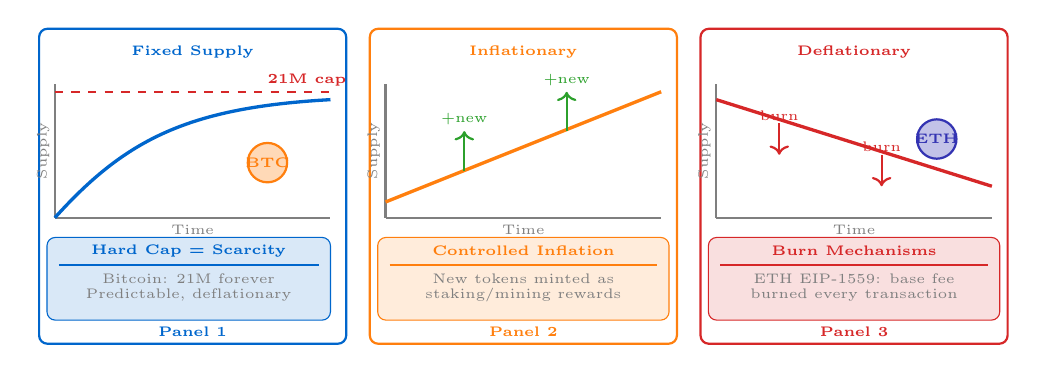
\begin{tikzpicture}
  % Panel borders
  \draw[thick, mlblue,   rounded corners=3pt] (0.1,0.2) rectangle (4.0,4.2);
  \draw[thick, mlorange, rounded corners=3pt] (4.3,0.2) rectangle (8.2,4.2);
  \draw[thick, mlred,    rounded corners=3pt] (8.5,0.2) rectangle (12.4,4.2);

  % --- Panel 1: Fixed Supply (Bitcoin) ---
  \node[font=\tiny\bfseries, mlblue] at (2.05,3.9) {Fixed Supply};
  % Flat line chart
  \draw[thick, mlgray] (0.3,1.8) -- (0.3,3.5);
  \draw[thick, mlgray] (0.3,1.8) -- (3.8,1.8);
  \node[font=\tiny, mlgray, rotate=90] at (0.15,2.65) {Supply};
  \node[font=\tiny, mlgray] at (2.05,1.65) {Time};
  % Supply curve that plateaus
  \draw[very thick, mlblue] (0.3,1.8) .. controls (1.2,2.8) and (2.0,3.2) .. (3.8,3.3);
  % Cap line
  \draw[dashed, thick, mlred] (0.3,3.4) -- (3.8,3.4);
  \node[font=\tiny\bfseries, mlred] at (3.5,3.55) {21M cap};
  % Bitcoin icon
  \draw[fill=mlorange!30, draw=mlorange, thick] (3.0,2.5) circle (0.25);
  \node[font=\tiny\bfseries, mlorange] at (3.0,2.5) {BTC};
  % Description
  \draw[fill=mlblue!15, draw=mlblue, rounded corners=3pt] (0.2,0.5) rectangle (3.8,1.55);
  \node[font=\tiny\bfseries, mlblue, align=center] at (2.0,1.38) {Hard Cap = Scarcity};
  \draw[mlblue, thin] (0.35,1.2) -- (3.65,1.2);
  \node[font=\tiny, mlgray, align=center] at (2.0,1.02) {Bitcoin: 21M forever};
  \node[font=\tiny, mlgray, align=center] at (2.0,0.82) {Predictable, deflationary};
  \node[font=\tiny\bfseries, mlblue] at (2.05,0.35) {Panel 1};

  % --- Panel 2: Inflationary (Ethereum PoS) ---
  \node[font=\tiny\bfseries, mlorange] at (6.25,3.9) {Inflationary};
  % Rising line chart
  \draw[thick, mlgray] (4.5,1.8) -- (4.5,3.5);
  \draw[thick, mlgray] (4.5,1.8) -- (8.0,1.8);
  \node[font=\tiny, mlgray, rotate=90] at (4.35,2.65) {Supply};
  \node[font=\tiny, mlgray] at (6.25,1.65) {Time};
  % Rising supply line
  \draw[very thick, mlorange] (4.5,2.0) -- (8.0,3.4);
  % Arrows showing new tokens
  \draw[->, thick, mlgreen] (5.5,2.4) -- (5.5,2.9);
  \node[font=\tiny, mlgreen] at (5.5,3.05) {+new};
  \draw[->, thick, mlgreen] (6.8,2.9) -- (6.8,3.4);
  \node[font=\tiny, mlgreen] at (6.8,3.55) {+new};
  % Description
  \draw[fill=mlorange!15, draw=mlorange, rounded corners=3pt] (4.4,0.5) rectangle (8.1,1.55);
  \node[font=\tiny\bfseries, mlorange, align=center] at (6.25,1.38) {Controlled Inflation};
  \draw[mlorange, thin] (4.55,1.2) -- (7.95,1.2);
  \node[font=\tiny, mlgray, align=center] at (6.25,1.02) {New tokens minted as};
  \node[font=\tiny, mlgray, align=center] at (6.25,0.82) {staking/mining rewards};
  \node[font=\tiny\bfseries, mlorange] at (6.25,0.35) {Panel 2};

  % --- Panel 3: Deflationary (ETH post-EIP-1559) ---
  \node[font=\tiny\bfseries, mlred] at (10.45,3.9) {Deflationary};
  % Declining line chart
  \draw[thick, mlgray] (8.7,1.8) -- (8.7,3.5);
  \draw[thick, mlgray] (8.7,1.8) -- (12.2,1.8);
  \node[font=\tiny, mlgray, rotate=90] at (8.55,2.65) {Supply};
  \node[font=\tiny, mlgray] at (10.45,1.65) {Time};
  % Declining supply line
  \draw[very thick, mlred] (8.7,3.3) -- (12.2,2.2);
  % Fire icons (burns)
  \node[font=\tiny, mlred] at (9.5,3.1) {burn};
  \draw[->, thick, mlred] (9.5,3.0) -- (9.5,2.6);
  \node[font=\tiny, mlred] at (10.8,2.7) {burn};
  \draw[->, thick, mlred] (10.8,2.6) -- (10.8,2.2);
  % ETH icon
  \draw[fill=mlpurple!30, draw=mlpurple, thick] (11.5,2.8) circle (0.25);
  \node[font=\tiny\bfseries, mlpurple] at (11.5,2.8) {ETH};
  % Description
  \draw[fill=mlred!15, draw=mlred, rounded corners=3pt] (8.6,0.5) rectangle (12.3,1.55);
  \node[font=\tiny\bfseries, mlred, align=center] at (10.45,1.38) {Burn Mechanisms};
  \draw[mlred, thin] (8.75,1.2) -- (12.15,1.2);
  \node[font=\tiny, mlgray, align=center] at (10.45,1.02) {ETH EIP-1559: base fee};
  \node[font=\tiny, mlgray, align=center] at (10.45,0.82) {burned every transaction};
  \node[font=\tiny\bfseries, mlred] at (10.45,0.35) {Panel 3};
\end{tikzpicture}

\bottomnote{Three supply models: Fixed (Bitcoin's 21M cap creates digital scarcity), Inflationary (new tokens minted as rewards, diluting holders), Deflationary (tokens burned, reducing supply over time like ETH post-EIP-1559).}
\end{frame}

% Frame 4: Token Utility Types
\begin{frame}{Token Utility Types}
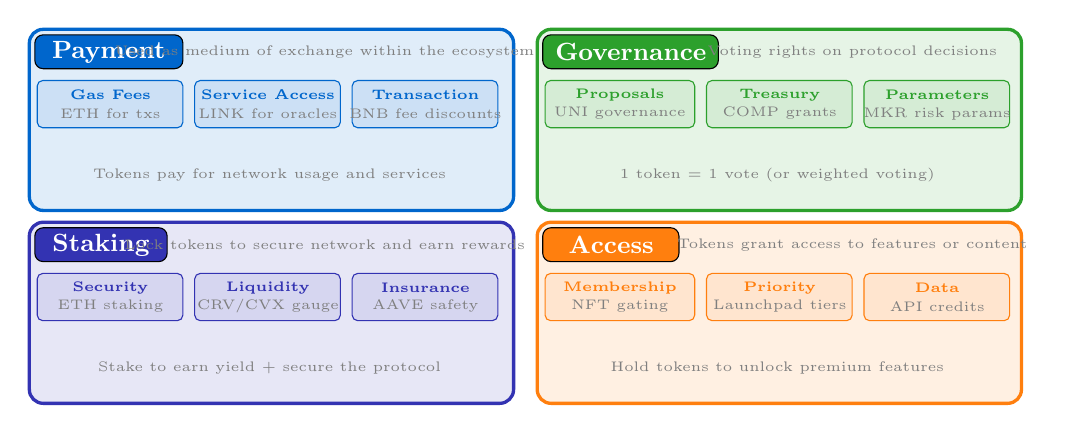
\begin{tikzpicture}
  % Four quadrants
  % Top-left: Payment
  \draw[fill=mlblue!12, draw=mlblue, very thick, rounded corners=5pt] (0.05,2.55) rectangle (6.2,4.85);
  \draw[fill=mlblue, rounded corners=3pt] (0.12,4.35) rectangle (2.0,4.78);
  \node[font=\small\bfseries, white, align=center] at (1.06,4.56) {Payment};
  \node[font=\tiny, mlgray, align=center] at (3.8,4.56) {Used as medium of exchange within the ecosystem};
  % Payment examples
  \draw[fill=mlblue!20, draw=mlblue, rounded corners=2pt] (0.15,3.6) rectangle (2.0,4.2);
  \node[font=\tiny\bfseries, mlblue, align=center] at (1.08,4.02) {Gas Fees};
  \node[font=\tiny, mlgray, align=center] at (1.08,3.78) {ETH for txs};
  \draw[fill=mlblue!20, draw=mlblue, rounded corners=2pt] (2.15,3.6) rectangle (4.0,4.2);
  \node[font=\tiny\bfseries, mlblue, align=center] at (3.08,4.02) {Service Access};
  \node[font=\tiny, mlgray, align=center] at (3.08,3.78) {LINK for oracles};
  \draw[fill=mlblue!20, draw=mlblue, rounded corners=2pt] (4.15,3.6) rectangle (6.0,4.2);
  \node[font=\tiny\bfseries, mlblue, align=center] at (5.08,4.02) {Transaction};
  \node[font=\tiny, mlgray, align=center] at (5.08,3.78) {BNB fee discounts};
  \node[font=\tiny, mlgray, align=center] at (3.1,3.0) {Tokens pay for network usage and services};

  % Top-right: Governance
  \draw[fill=mlgreen!12, draw=mlgreen, very thick, rounded corners=5pt] (6.5,2.55) rectangle (12.65,4.85);
  \draw[fill=mlgreen, rounded corners=3pt] (6.57,4.35) rectangle (8.8,4.78);
  \node[font=\small\bfseries, white, align=center] at (7.69,4.56) {Governance};
  \node[font=\tiny, mlgray, align=center] at (10.5,4.56) {Voting rights on protocol decisions};
  \draw[fill=mlgreen!20, draw=mlgreen, rounded corners=2pt] (6.6,3.6) rectangle (8.5,4.2);
  \node[font=\tiny\bfseries, mlgreen, align=center] at (7.55,4.02) {Proposals};
  \node[font=\tiny, mlgray, align=center] at (7.55,3.78) {UNI governance};
  \draw[fill=mlgreen!20, draw=mlgreen, rounded corners=2pt] (8.65,3.6) rectangle (10.5,4.2);
  \node[font=\tiny\bfseries, mlgreen, align=center] at (9.58,4.02) {Treasury};
  \node[font=\tiny, mlgray, align=center] at (9.58,3.78) {COMP grants};
  \draw[fill=mlgreen!20, draw=mlgreen, rounded corners=2pt] (10.65,3.6) rectangle (12.5,4.2);
  \node[font=\tiny\bfseries, mlgreen, align=center] at (11.58,4.02) {Parameters};
  \node[font=\tiny, mlgray, align=center] at (11.58,3.78) {MKR risk params};
  \node[font=\tiny, mlgray, align=center] at (9.55,3.0) {1 token = 1 vote (or weighted voting)};

  % Bottom-left: Staking
  \draw[fill=mlpurple!12, draw=mlpurple, very thick, rounded corners=5pt] (0.05,0.1) rectangle (6.2,2.4);
  \draw[fill=mlpurple, rounded corners=3pt] (0.12,1.9) rectangle (1.8,2.33);
  \node[font=\small\bfseries, white, align=center] at (0.96,2.11) {Staking};
  \node[font=\tiny, mlgray, align=center] at (3.8,2.11) {Lock tokens to secure network and earn rewards};
  \draw[fill=mlpurple!20, draw=mlpurple, rounded corners=2pt] (0.15,1.15) rectangle (2.0,1.75);
  \node[font=\tiny\bfseries, mlpurple, align=center] at (1.08,1.57) {Security};
  \node[font=\tiny, mlgray, align=center] at (1.08,1.33) {ETH staking};
  \draw[fill=mlpurple!20, draw=mlpurple, rounded corners=2pt] (2.15,1.15) rectangle (4.0,1.75);
  \node[font=\tiny\bfseries, mlpurple, align=center] at (3.08,1.57) {Liquidity};
  \node[font=\tiny, mlgray, align=center] at (3.08,1.33) {CRV/CVX gauge};
  \draw[fill=mlpurple!20, draw=mlpurple, rounded corners=2pt] (4.15,1.15) rectangle (6.0,1.75);
  \node[font=\tiny\bfseries, mlpurple, align=center] at (5.08,1.57) {Insurance};
  \node[font=\tiny, mlgray, align=center] at (5.08,1.33) {AAVE safety};
  \node[font=\tiny, mlgray, align=center] at (3.1,0.55) {Stake to earn yield + secure the protocol};

  % Bottom-right: Access
  \draw[fill=mlorange!12, draw=mlorange, very thick, rounded corners=5pt] (6.5,0.1) rectangle (12.65,2.4);
  \draw[fill=mlorange, rounded corners=3pt] (6.57,1.9) rectangle (8.3,2.33);
  \node[font=\small\bfseries, white, align=center] at (7.44,2.11) {Access};
  \node[font=\tiny, mlgray, align=center] at (10.5,2.11) {Tokens grant access to features or content};
  \draw[fill=mlorange!20, draw=mlorange, rounded corners=2pt] (6.6,1.15) rectangle (8.5,1.75);
  \node[font=\tiny\bfseries, mlorange, align=center] at (7.55,1.57) {Membership};
  \node[font=\tiny, mlgray, align=center] at (7.55,1.33) {NFT gating};
  \draw[fill=mlorange!20, draw=mlorange, rounded corners=2pt] (8.65,1.15) rectangle (10.5,1.75);
  \node[font=\tiny\bfseries, mlorange, align=center] at (9.58,1.57) {Priority};
  \node[font=\tiny, mlgray, align=center] at (9.58,1.33) {Launchpad tiers};
  \draw[fill=mlorange!20, draw=mlorange, rounded corners=2pt] (10.65,1.15) rectangle (12.5,1.75);
  \node[font=\tiny\bfseries, mlorange, align=center] at (11.58,1.57) {Data};
  \node[font=\tiny, mlgray, align=center] at (11.58,1.33) {API credits};
  \node[font=\tiny, mlgray, align=center] at (9.55,0.55) {Hold tokens to unlock premium features};
\end{tikzpicture}

\bottomnote{Four main token utility types: Payment (gas fees, services), Governance (voting on proposals, parameters, treasury), Staking (lock tokens for security and yield), Access (gate content, priority, or features).}
\end{frame}

% Frame 5: Bonding Curves Visualized
\begin{frame}{Bonding Curves Visualized}
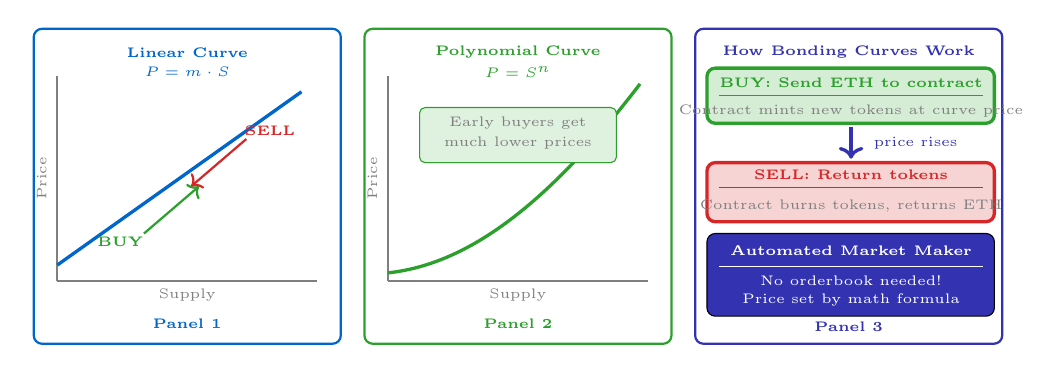
\begin{tikzpicture}
  % Panel borders
  \draw[thick, mlblue,   rounded corners=3pt] (0.1,0.2) rectangle (4.0,4.2);
  \draw[thick, mlgreen,  rounded corners=3pt] (4.3,0.2) rectangle (8.2,4.2);
  \draw[thick, mlpurple, rounded corners=3pt] (8.5,0.2) rectangle (12.4,4.2);

  % --- Panel 1: Linear Bonding Curve ---
  \node[font=\tiny\bfseries, mlblue] at (2.05,3.9) {Linear Curve};
  % Axes
  \draw[thick, mlgray] (0.4,1.0) -- (0.4,3.6);
  \draw[thick, mlgray] (0.4,1.0) -- (3.7,1.0);
  \node[font=\tiny, mlgray, rotate=90] at (0.2,2.3) {Price};
  \node[font=\tiny, mlgray] at (2.05,0.82) {Supply};
  % Linear line
  \draw[very thick, mlblue] (0.4,1.2) -- (3.5,3.4);
  % Formula
  \node[font=\tiny, mlblue] at (2.05,3.65) {$P = m \cdot S$};
  % Buy/sell arrows
  \draw[->, thick, mlgreen] (1.5,1.6) -- (2.2,2.2);
  \node[font=\tiny\bfseries, mlgreen] at (1.2,1.5) {BUY};
  \draw[->, thick, mlred] (2.8,2.8) -- (2.1,2.2);
  \node[font=\tiny\bfseries, mlred] at (3.1,2.9) {SELL};
  \node[font=\tiny\bfseries, mlblue] at (2.05,0.45) {Panel 1};

  % --- Panel 2: Polynomial Curve ---
  \node[font=\tiny\bfseries, mlgreen] at (6.25,3.9) {Polynomial Curve};
  % Axes
  \draw[thick, mlgray] (4.6,1.0) -- (4.6,3.6);
  \draw[thick, mlgray] (4.6,1.0) -- (7.9,1.0);
  \node[font=\tiny, mlgray, rotate=90] at (4.4,2.3) {Price};
  \node[font=\tiny, mlgray] at (6.25,0.82) {Supply};
  % Polynomial curve (quadratic)
  \draw[very thick, mlgreen] (4.6,1.1) .. controls (5.5,1.2) and (6.5,1.8) .. (7.8,3.5);
  % Formula
  \node[font=\tiny, mlgreen] at (6.25,3.65) {$P = S^n$};
  % Annotation
  \draw[fill=mlgreen!15, draw=mlgreen, rounded corners=2pt] (5.0,2.5) rectangle (7.5,3.2);
  \node[font=\tiny, mlgray, align=center] at (6.25,3.0) {Early buyers get};
  \node[font=\tiny, mlgray, align=center] at (6.25,2.75) {much lower prices};
  \node[font=\tiny\bfseries, mlgreen] at (6.25,0.45) {Panel 2};

  % --- Panel 3: How It Works ---
  \node[font=\tiny\bfseries, mlpurple] at (10.45,3.9) {How Bonding Curves Work};
  % Buy flow
  \draw[fill=mlgreen!20, draw=mlgreen, very thick, rounded corners=3pt] (8.65,3.0) rectangle (12.3,3.7);
  \node[font=\tiny\bfseries, mlgreen, align=center] at (10.48,3.52) {BUY: Send ETH to contract};
  \draw[mlgreen, thin] (8.8,3.35) -- (12.15,3.35);
  \node[font=\tiny, mlgray, align=center] at (10.48,3.15) {Contract mints new tokens at curve price};
  % Arrow
  \draw[->, very thick, mlpurple] (10.48,2.95) -- (10.48,2.55);
  \node[font=\tiny, mlpurple] at (11.3,2.75) {price rises};
  % Sell flow
  \draw[fill=mlred!20, draw=mlred, very thick, rounded corners=3pt] (8.65,1.75) rectangle (12.3,2.5);
  \node[font=\tiny\bfseries, mlred, align=center] at (10.48,2.35) {SELL: Return tokens};
  \draw[mlred, thin] (8.8,2.18) -- (12.15,2.18);
  \node[font=\tiny, mlgray, align=center] at (10.48,1.95) {Contract burns tokens, returns ETH};
  % Key point
  \draw[fill=mlpurple, rounded corners=3pt] (8.65,0.55) rectangle (12.3,1.6);
  \node[font=\tiny\bfseries, white, align=center] at (10.48,1.38) {Automated Market Maker};
  \draw[white, thin] (8.8,1.18) -- (12.15,1.18);
  \node[font=\tiny, white, align=center] at (10.48,1.0) {No orderbook needed!};
  \node[font=\tiny, white, align=center] at (10.48,0.75) {Price set by math formula};
  \node[font=\tiny\bfseries, mlpurple] at (10.45,0.42) {Panel 3};
\end{tikzpicture}

\bottomnote{Bonding curves are mathematical functions that set token price based on supply. Buy = mint tokens (price increases). Sell = burn tokens (price decreases). No orderbook -- the smart contract IS the market maker.}
\end{frame}

% Frame 6: Incentive Alignment
\begin{frame}{Incentive Alignment \& Game Theory}
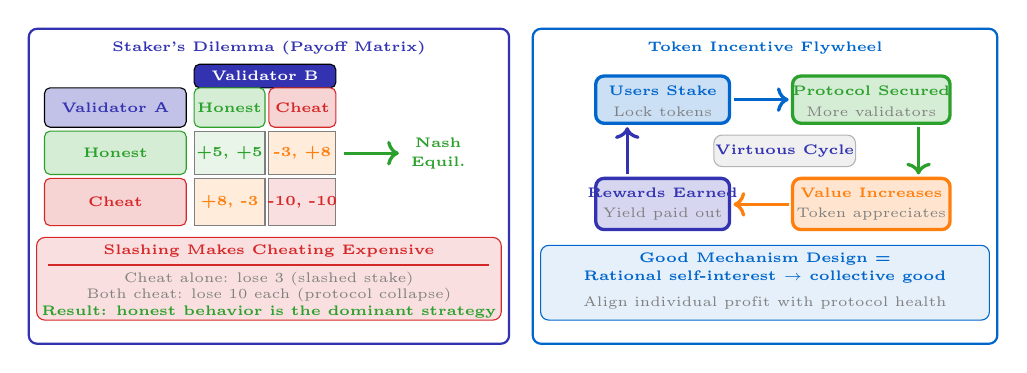
\begin{tikzpicture}
  % Panel borders
  \draw[thick, mlpurple, rounded corners=3pt] (0.1,0.2) rectangle (6.2,4.2);
  \draw[thick, mlblue,   rounded corners=3pt] (6.5,0.2) rectangle (12.4,4.2);

  % --- Left Panel: Payoff Matrix ---
  \node[font=\tiny\bfseries, mlpurple] at (3.15,3.95) {Staker's Dilemma (Payoff Matrix)};

  % Matrix headers
  \draw[fill=mlpurple, rounded corners=2pt] (2.2,3.45) rectangle (4.0,3.75);
  \node[font=\tiny\bfseries, white] at (3.1,3.6) {Validator B};
  \draw[fill=mlpurple!30, rounded corners=2pt] (0.3,2.95) rectangle (2.1,3.45);
  \node[font=\tiny\bfseries, mlpurple, align=center] at (1.2,3.2) {Validator A};

  % Column headers
  \draw[fill=mlgreen!20, draw=mlgreen, rounded corners=2pt] (2.2,2.95) rectangle (3.1,3.45);
  \node[font=\tiny\bfseries, mlgreen, align=center] at (2.65,3.2) {Honest};
  \draw[fill=mlred!20, draw=mlred, rounded corners=2pt] (3.15,2.95) rectangle (4.0,3.45);
  \node[font=\tiny\bfseries, mlred, align=center] at (3.575,3.2) {Cheat};

  % Row headers
  \draw[fill=mlgreen!20, draw=mlgreen, rounded corners=2pt] (0.3,2.35) rectangle (2.1,2.9);
  \node[font=\tiny\bfseries, mlgreen, align=center] at (1.2,2.62) {Honest};
  \draw[fill=mlred!20, draw=mlred, rounded corners=2pt] (0.3,1.7) rectangle (2.1,2.3);
  \node[font=\tiny\bfseries, mlred, align=center] at (1.2,2.0) {Cheat};

  % Payoff cells
  \draw[fill=mlgreen!10, draw=mlgray] (2.2,2.35) rectangle (3.1,2.9);
  \node[font=\tiny\bfseries, mlgreen, align=center] at (2.65,2.62) {+5, +5};
  \draw[fill=mlorange!15, draw=mlgray] (3.15,2.35) rectangle (4.0,2.9);
  \node[font=\tiny\bfseries, mlorange, align=center] at (3.575,2.62) {-3, +8};
  \draw[fill=mlorange!15, draw=mlgray] (2.2,1.7) rectangle (3.1,2.3);
  \node[font=\tiny\bfseries, mlorange, align=center] at (2.65,2.0) {+8, -3};
  \draw[fill=mlred!15, draw=mlgray] (3.15,1.7) rectangle (4.0,2.3);
  \node[font=\tiny\bfseries, mlred, align=center] at (3.575,2.0) {-10, -10};

  % Arrow pointing to Nash equilibrium
  \draw[->, very thick, mlgreen] (4.1,2.62) -- (4.8,2.62);
  \node[font=\tiny\bfseries, mlgreen, align=center] at (5.3,2.75) {Nash};
  \node[font=\tiny\bfseries, mlgreen, align=center] at (5.3,2.5) {Equil.};

  % Slashing explanation
  \draw[fill=mlred!15, draw=mlred, rounded corners=3pt] (0.2,0.5) rectangle (6.1,1.55);
  \node[font=\tiny\bfseries, mlred, align=center] at (3.15,1.38) {Slashing Makes Cheating Expensive};
  \draw[mlred, thin] (0.35,1.2) -- (5.95,1.2);
  \node[font=\tiny, mlgray, align=center] at (3.15,1.02) {Cheat alone: lose 3 (slashed stake)};
  \node[font=\tiny, mlgray, align=center] at (3.15,0.82) {Both cheat: lose 10 each (protocol collapse)};
  \node[font=\tiny\bfseries, mlgreen, align=center] at (3.15,0.6) {Result: honest behavior is the dominant strategy};

  % --- Right Panel: Incentive Loop ---
  \node[font=\tiny\bfseries, mlblue] at (9.45,3.95) {Token Incentive Flywheel};
  % Circular flow
  \draw[fill=mlblue!20, draw=mlblue, very thick, rounded corners=3pt] (7.3,3.0) rectangle (9.0,3.6);
  \node[font=\tiny\bfseries, mlblue, align=center] at (8.15,3.42) {Users Stake};
  \node[font=\tiny, mlgray, align=center] at (8.15,3.15) {Lock tokens};

  \draw[fill=mlgreen!20, draw=mlgreen, very thick, rounded corners=3pt] (9.8,3.0) rectangle (11.8,3.6);
  \node[font=\tiny\bfseries, mlgreen, align=center] at (10.8,3.42) {Protocol Secured};
  \node[font=\tiny, mlgray, align=center] at (10.8,3.15) {More validators};

  \draw[fill=mlorange!20, draw=mlorange, very thick, rounded corners=3pt] (9.8,1.65) rectangle (11.8,2.3);
  \node[font=\tiny\bfseries, mlorange, align=center] at (10.8,2.12) {Value Increases};
  \node[font=\tiny, mlgray, align=center] at (10.8,1.85) {Token appreciates};

  \draw[fill=mlpurple!20, draw=mlpurple, very thick, rounded corners=3pt] (7.3,1.65) rectangle (9.0,2.3);
  \node[font=\tiny\bfseries, mlpurple, align=center] at (8.15,2.12) {Rewards Earned};
  \node[font=\tiny, mlgray, align=center] at (8.15,1.85) {Yield paid out};

  % Circular arrows
  \draw[->, very thick, mlblue] (9.05,3.3) -- (9.75,3.3);
  \draw[->, very thick, mlgreen] (11.4,2.95) -- (11.4,2.35);
  \draw[->, very thick, mlorange] (9.75,1.97) -- (9.05,1.97);
  \draw[->, very thick, mlpurple] (7.7,2.35) -- (7.7,2.95);

  % Center label
  \draw[fill=lightgray, draw=midgray, rounded corners=3pt] (8.8,2.45) rectangle (10.6,2.85);
  \node[font=\tiny\bfseries, mlpurple, align=center] at (9.7,2.65) {Virtuous Cycle};

  % Bottom summary
  \draw[fill=mlblue!10, draw=mlblue, rounded corners=3pt] (6.6,0.5) rectangle (12.3,1.45);
  \node[font=\tiny\bfseries, mlblue, align=center] at (9.45,1.28) {Good Mechanism Design =};
  \node[font=\tiny\bfseries, mlblue, align=center] at (9.45,1.05) {Rational self-interest $\to$ collective good};
  \node[font=\tiny, mlgray, align=center] at (9.45,0.72) {Align individual profit with protocol health};
\end{tikzpicture}

\bottomnote{Good tokenomics uses game theory: slashing makes dishonesty unprofitable (Nash equilibrium favors honest behavior). The incentive flywheel creates a virtuous cycle: stake $\to$ secure $\to$ value up $\to$ rewards $\to$ more staking.}
\end{frame}

% Frame 7: Token Distribution
\begin{frame}{Token Distribution}
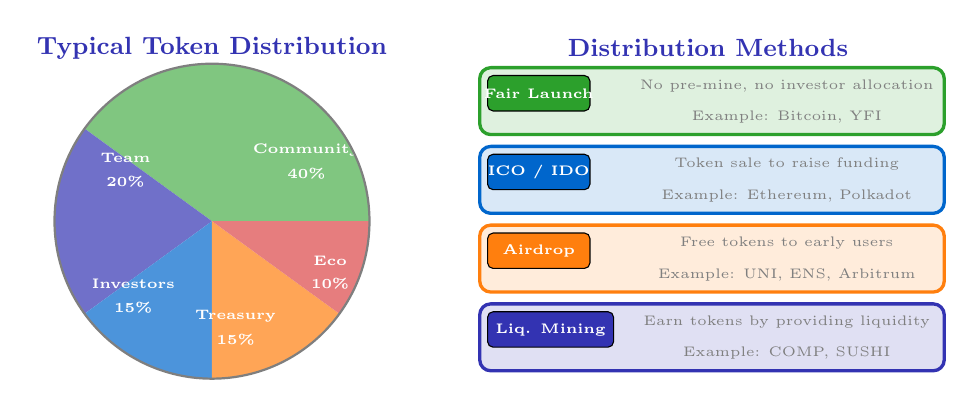
\begin{tikzpicture}
  % --- Left: Pie Chart ---
  % Title
  \node[font=\small\bfseries, mlpurple] at (3.2,4.7) {Typical Token Distribution};

  % Pie chart center
  \def\cx{3.2}
  \def\cy{2.5}
  \def\radius{2.0}

  % Community (40%) - green - 0 to 144 degrees
  \fill[mlgreen!60] (\cx,\cy) -- ++(0:\radius) arc (0:144:\radius) -- cycle;
  \node[font=\tiny\bfseries, white] at ($({\cx+1.2},{\cy+0.9})$) {Community};
  \node[font=\tiny\bfseries, white] at ($({\cx+1.2},{\cy+0.6})$) {40\%};

  % Team (20%) - purple - 144 to 216 degrees
  \fill[mlpurple!70] (\cx,\cy) -- ++(144:\radius) arc (144:216:\radius) -- cycle;
  \node[font=\tiny\bfseries, white] at ($({\cx-1.1},{\cy+0.8})$) {Team};
  \node[font=\tiny\bfseries, white] at ($({\cx-1.1},{\cy+0.5})$) {20\%};

  % Investors (15%) - blue - 216 to 270 degrees
  \fill[mlblue!70] (\cx,\cy) -- ++(216:\radius) arc (216:270:\radius) -- cycle;
  \node[font=\tiny\bfseries, white] at ($({\cx-1.0},{\cy-0.8})$) {Investors};
  \node[font=\tiny\bfseries, white] at ($({\cx-1.0},{\cy-1.1})$) {15\%};

  % Treasury (15%) - orange - 270 to 324 degrees
  \fill[mlorange!70] (\cx,\cy) -- ++(270:\radius) arc (270:324:\radius) -- cycle;
  \node[font=\tiny\bfseries, white] at ($({\cx+0.3},{\cy-1.2})$) {Treasury};
  \node[font=\tiny\bfseries, white] at ($({\cx+0.3},{\cy-1.5})$) {15\%};

  % Ecosystem (10%) - red - 324 to 360 degrees
  \fill[mlred!60] (\cx,\cy) -- ++(324:\radius) arc (324:360:\radius) -- cycle;
  \node[font=\tiny\bfseries, white] at ($({\cx+1.5},{\cy-0.5})$) {Eco};
  \node[font=\tiny\bfseries, white] at ($({\cx+1.5},{\cy-0.8})$) {10\%};

  % Outline
  \draw[thick, mlgray] (\cx,\cy) circle (\radius);

  % --- Right: Distribution Methods ---
  \node[font=\small\bfseries, mlpurple] at (9.5,4.7) {Distribution Methods};

  % Method 1: Fair Launch
  \draw[fill=mlgreen!15, draw=mlgreen, very thick, rounded corners=4pt] (6.6,3.6) rectangle (12.5,4.45);
  \draw[fill=mlgreen, rounded corners=2pt] (6.7,3.9) rectangle (8.0,4.35);
  \node[font=\tiny\bfseries, white, align=center] at (7.35,4.12) {Fair Launch};
  \node[font=\tiny, mlgray, align=center] at (10.5,4.22) {No pre-mine, no investor allocation};
  \node[font=\tiny, mlgray, align=center] at (10.5,3.82) {Example: Bitcoin, YFI};

  % Method 2: ICO/IDO
  \draw[fill=mlblue!15, draw=mlblue, very thick, rounded corners=4pt] (6.6,2.6) rectangle (12.5,3.45);
  \draw[fill=mlblue, rounded corners=2pt] (6.7,2.9) rectangle (8.0,3.35);
  \node[font=\tiny\bfseries, white, align=center] at (7.35,3.12) {ICO / IDO};
  \node[font=\tiny, mlgray, align=center] at (10.5,3.22) {Token sale to raise funding};
  \node[font=\tiny, mlgray, align=center] at (10.5,2.82) {Example: Ethereum, Polkadot};

  % Method 3: Airdrop
  \draw[fill=mlorange!15, draw=mlorange, very thick, rounded corners=4pt] (6.6,1.6) rectangle (12.5,2.45);
  \draw[fill=mlorange, rounded corners=2pt] (6.7,1.9) rectangle (8.0,2.35);
  \node[font=\tiny\bfseries, white, align=center] at (7.35,2.12) {Airdrop};
  \node[font=\tiny, mlgray, align=center] at (10.5,2.22) {Free tokens to early users};
  \node[font=\tiny, mlgray, align=center] at (10.5,1.82) {Example: UNI, ENS, Arbitrum};

  % Method 4: Liquidity Mining
  \draw[fill=mlpurple!15, draw=mlpurple, very thick, rounded corners=4pt] (6.6,0.6) rectangle (12.5,1.45);
  \draw[fill=mlpurple, rounded corners=2pt] (6.7,0.9) rectangle (8.3,1.35);
  \node[font=\tiny\bfseries, white, align=center] at (7.5,1.12) {Liq. Mining};
  \node[font=\tiny, mlgray, align=center] at (10.5,1.22) {Earn tokens by providing liquidity};
  \node[font=\tiny, mlgray, align=center] at (10.5,0.82) {Example: COMP, SUSHI};
\end{tikzpicture}

\bottomnote{Token distribution determines who holds tokens and when. Typical split: 40\% community, 20\% team, 15\% investors, 15\% treasury, 10\% ecosystem. Methods: fair launch (no pre-mine), ICO/IDO (sale), airdrop (free to users), liquidity mining.}
\end{frame}

% Frame 8: Vesting & Unlock Schedules
\begin{frame}{Vesting \& Unlock Schedules}
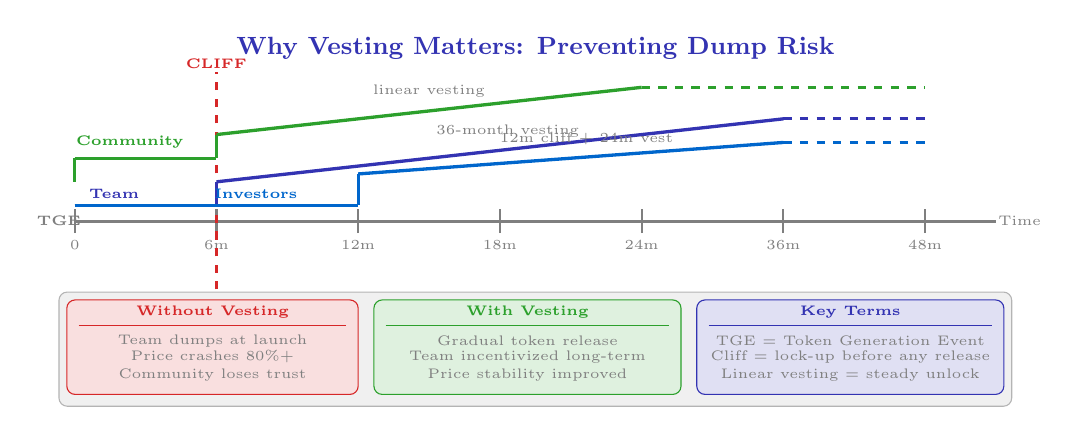
\begin{tikzpicture}
  % Title area
  \node[font=\small\bfseries, mlpurple] at (6.35,4.7) {Why Vesting Matters: Preventing Dump Risk};

  % Timeline axis
  \draw[very thick, mlgray] (0.5,2.5) -- (12.2,2.5);
  \node[font=\tiny\bfseries, mlgray] at (0.3,2.5) {TGE};
  \node[font=\tiny, mlgray] at (12.5,2.5) {Time};

  % Time markers
  \foreach \x/\label in {0.5/0, 2.3/6m, 4.1/12m, 5.9/18m, 7.7/24m, 9.5/36m, 11.3/48m} {
    \draw[thick, mlgray] (\x,2.35) -- (\x,2.65);
    \node[font=\tiny, mlgray] at (\x,2.2) {\label};
  }

  % Cliff marker
  \draw[very thick, mlred, dashed] (2.3,1.0) -- (2.3,4.4);
  \node[font=\tiny\bfseries, mlred] at (2.3,4.5) {CLIFF};
  \node[font=\tiny, mlgray] at (2.3,0.8) {6-month cliff};

  % Community tokens (green) - immediate partial + vesting
  \draw[very thick, mlgreen] (0.5,3.0) -- (0.5,3.3);
  \draw[very thick, mlgreen] (0.5,3.3) -- (2.3,3.3);
  \draw[very thick, mlgreen] (2.3,3.3) -- (2.3,3.6);
  \draw[very thick, mlgreen] (2.3,3.6) -- (7.7,4.2);
  \draw[very thick, mlgreen, dashed] (7.7,4.2) -- (11.3,4.2);
  \node[font=\tiny\bfseries, mlgreen] at (1.2,3.5) {Community};
  \node[font=\tiny, mlgray] at (5.0,4.15) {linear vesting};

  % Team tokens (purple) - full cliff then vesting
  \draw[very thick, mlpurple] (0.5,2.7) -- (2.3,2.7);
  \draw[very thick, mlpurple] (2.3,2.7) -- (2.3,3.0);
  \draw[very thick, mlpurple] (2.3,3.0) -- (9.5,3.8);
  \draw[very thick, mlpurple, dashed] (9.5,3.8) -- (11.3,3.8);
  \node[font=\tiny\bfseries, mlpurple] at (1.0,2.85) {Team};
  \node[font=\tiny, mlgray] at (6.0,3.65) {36-month vesting};

  % Investor tokens (blue) - cliff then shorter vesting
  \draw[very thick, mlblue] (0.5,2.7) -- (4.1,2.7);
  \draw[very thick, mlblue] (4.1,2.7) -- (4.1,3.1);
  \draw[very thick, mlblue] (4.1,3.1) -- (9.5,3.5);
  \draw[very thick, mlblue, dashed] (9.5,3.5) -- (11.3,3.5);
  \node[font=\tiny\bfseries, mlblue] at (2.8,2.85) {Investors};
  \node[font=\tiny, mlgray] at (7.0,3.55) {12m cliff + 24m vest};

  % Legend
  \draw[fill=lightgray, draw=midgray, rounded corners=3pt] (0.3,0.15) rectangle (12.4,1.6);
  % No vesting column
  \draw[fill=mlred!15, draw=mlred, rounded corners=3pt] (0.4,0.3) rectangle (4.1,1.5);
  \node[font=\tiny\bfseries, mlred, align=center] at (2.25,1.35) {Without Vesting};
  \draw[mlred, thin] (0.55,1.18) -- (3.95,1.18);
  \node[font=\tiny, mlgray, align=center] at (2.25,0.98) {Team dumps at launch};
  \node[font=\tiny, mlgray, align=center] at (2.25,0.78) {Price crashes 80\%+};
  \node[font=\tiny, mlgray, align=center] at (2.25,0.55) {Community loses trust};

  % With vesting column
  \draw[fill=mlgreen!15, draw=mlgreen, rounded corners=3pt] (4.3,0.3) rectangle (8.2,1.5);
  \node[font=\tiny\bfseries, mlgreen, align=center] at (6.25,1.35) {With Vesting};
  \draw[mlgreen, thin] (4.45,1.18) -- (8.05,1.18);
  \node[font=\tiny, mlgray, align=center] at (6.25,0.98) {Gradual token release};
  \node[font=\tiny, mlgray, align=center] at (6.25,0.78) {Team incentivized long-term};
  \node[font=\tiny, mlgray, align=center] at (6.25,0.55) {Price stability improved};

  % Key terms
  \draw[fill=mlpurple!15, draw=mlpurple, rounded corners=3pt] (8.4,0.3) rectangle (12.3,1.5);
  \node[font=\tiny\bfseries, mlpurple, align=center] at (10.35,1.35) {Key Terms};
  \draw[mlpurple, thin] (8.55,1.18) -- (12.15,1.18);
  \node[font=\tiny, mlgray, align=center] at (10.35,0.98) {TGE = Token Generation Event};
  \node[font=\tiny, mlgray, align=center] at (10.35,0.78) {Cliff = lock-up before any release};
  \node[font=\tiny, mlgray, align=center] at (10.35,0.55) {Linear vesting = steady unlock};
\end{tikzpicture}

\bottomnote{Vesting schedules prevent insiders from dumping tokens at launch. Typical: 6--12 month cliff (no tokens released), then 24--48 month linear vesting. Community tokens often have shorter or no cliff; team/investor tokens have longer lock-ups.}
\end{frame}

% Frame 9: Case Study: UNI vs MKR
\begin{frame}{Case Study: UNI vs MKR}
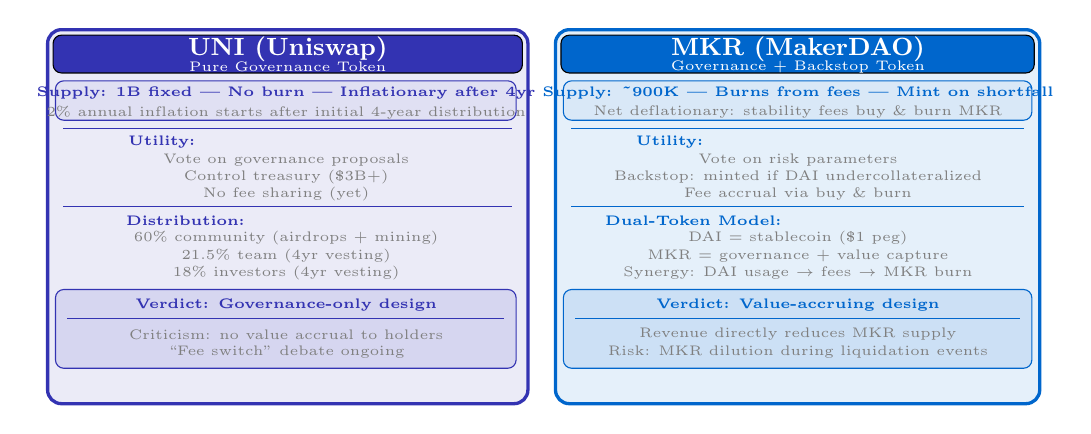
\begin{tikzpicture}
  % --- Left: UNI ---
  \draw[fill=mlpurple!10, draw=mlpurple, very thick, rounded corners=5pt] (0.05,0.1) rectangle (6.15,4.85);
  % Header
  \draw[fill=mlpurple, rounded corners=3pt] (0.12,4.3) rectangle (6.08,4.78);
  \node[font=\small\bfseries, white, align=center] at (3.1,4.6) {UNI (Uniswap)};
  \node[font=\tiny, white, align=center] at (3.1,4.38) {Pure Governance Token};

  % Supply info
  \draw[fill=mlpurple!15, draw=mlpurple, rounded corners=3pt] (0.15,3.7) rectangle (6.0,4.2);
  \node[font=\tiny\bfseries, mlpurple, align=center] at (3.08,4.05) {Supply: 1B fixed | No burn | Inflationary after 4yr};
  \node[font=\tiny, mlgray, align=center] at (3.08,3.8) {2\% annual inflation starts after initial 4-year distribution};

  % Utility
  \draw[mlpurple, thin] (0.25,3.6) -- (5.95,3.6);
  \node[font=\tiny\bfseries, mlpurple] at (1.5,3.42) {Utility:};
  \node[font=\tiny, mlgray, align=center] at (3.08,3.2) {Vote on governance proposals};
  \node[font=\tiny, mlgray, align=center] at (3.08,2.98) {Control treasury (\$3B+)};
  \node[font=\tiny, mlgray, align=center] at (3.08,2.76) {No fee sharing (yet)};

  % Distribution
  \draw[mlpurple, thin] (0.25,2.6) -- (5.95,2.6);
  \node[font=\tiny\bfseries, mlpurple] at (1.8,2.42) {Distribution:};
  \node[font=\tiny, mlgray, align=center] at (3.08,2.2) {60\% community (airdrops + mining)};
  \node[font=\tiny, mlgray, align=center] at (3.08,1.98) {21.5\% team (4yr vesting)};
  \node[font=\tiny, mlgray, align=center] at (3.08,1.76) {18\% investors (4yr vesting)};

  % Verdict
  \draw[fill=mlpurple!20, draw=mlpurple, rounded corners=3pt] (0.15,0.55) rectangle (6.0,1.55);
  \node[font=\tiny\bfseries, mlpurple, align=center] at (3.08,1.35) {Verdict: Governance-only design};
  \draw[mlpurple, thin] (0.3,1.18) -- (5.85,1.18);
  \node[font=\tiny, mlgray, align=center] at (3.08,0.98) {Criticism: no value accrual to holders};
  \node[font=\tiny, mlgray, align=center] at (3.08,0.75) {``Fee switch'' debate ongoing};

  % --- Right: MKR ---
  \draw[fill=mlblue!10, draw=mlblue, very thick, rounded corners=5pt] (6.5,0.1) rectangle (12.65,4.85);
  % Header
  \draw[fill=mlblue, rounded corners=3pt] (6.57,4.3) rectangle (12.58,4.78);
  \node[font=\small\bfseries, white, align=center] at (9.58,4.6) {MKR (MakerDAO)};
  \node[font=\tiny, white, align=center] at (9.58,4.38) {Governance + Backstop Token};

  % Supply info
  \draw[fill=mlblue!15, draw=mlblue, rounded corners=3pt] (6.6,3.7) rectangle (12.55,4.2);
  \node[font=\tiny\bfseries, mlblue, align=center] at (9.58,4.05) {Supply: \textasciitilde900K | Burns from fees | Mint on shortfall};
  \node[font=\tiny, mlgray, align=center] at (9.58,3.8) {Net deflationary: stability fees buy \& burn MKR};

  % Utility
  \draw[mlblue, thin] (6.7,3.6) -- (12.45,3.6);
  \node[font=\tiny\bfseries, mlblue] at (7.95,3.42) {Utility:};
  \node[font=\tiny, mlgray, align=center] at (9.58,3.2) {Vote on risk parameters};
  \node[font=\tiny, mlgray, align=center] at (9.58,2.98) {Backstop: minted if DAI undercollateralized};
  \node[font=\tiny, mlgray, align=center] at (9.58,2.76) {Fee accrual via buy \& burn};

  % Distribution
  \draw[mlblue, thin] (6.7,2.6) -- (12.45,2.6);
  \node[font=\tiny\bfseries, mlblue] at (8.25,2.42) {Dual-Token Model:};
  \node[font=\tiny, mlgray, align=center] at (9.58,2.2) {DAI = stablecoin (\$1 peg)};
  \node[font=\tiny, mlgray, align=center] at (9.58,1.98) {MKR = governance + value capture};
  \node[font=\tiny, mlgray, align=center] at (9.58,1.76) {Synergy: DAI usage $\to$ fees $\to$ MKR burn};

  % Verdict
  \draw[fill=mlblue!20, draw=mlblue, rounded corners=3pt] (6.6,0.55) rectangle (12.55,1.55);
  \node[font=\tiny\bfseries, mlblue, align=center] at (9.58,1.35) {Verdict: Value-accruing design};
  \draw[mlblue, thin] (6.75,1.18) -- (12.4,1.18);
  \node[font=\tiny, mlgray, align=center] at (9.58,0.98) {Revenue directly reduces MKR supply};
  \node[font=\tiny, mlgray, align=center] at (9.58,0.75) {Risk: MKR dilution during liquidation events};
\end{tikzpicture}

\bottomnote{UNI: pure governance token with no direct fee capture -- ``fee switch'' remains controversial. MKR: governance + value accrual via buy-and-burn from stability fees, but carries backstop dilution risk. Two contrasting approaches to token design.}
\end{frame}

% Frame 10: Key Takeaways
\begin{frame}{Key Takeaways}
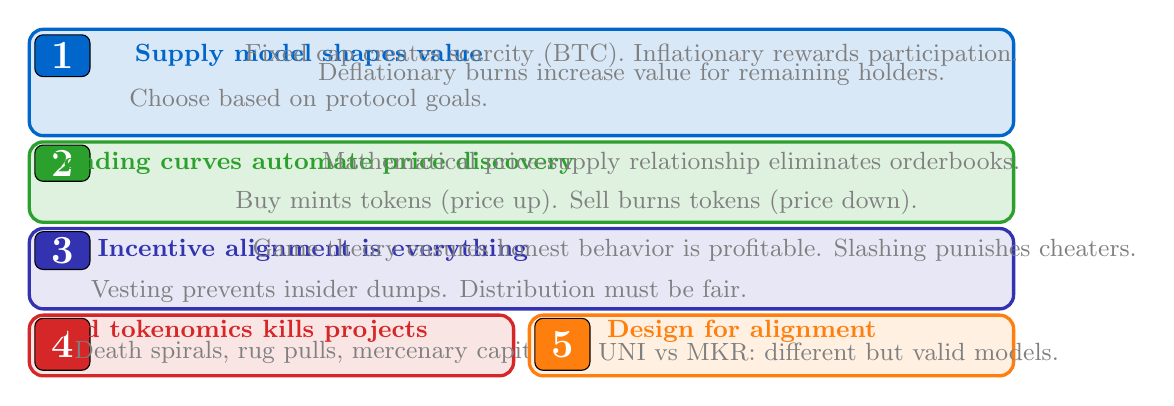
\begin{tikzpicture}
  % Box 1
  \draw[fill=mlblue!15, draw=mlblue, very thick, rounded corners=5pt] (0.05,3.2) rectangle (12.55,4.55);
  \draw[fill=mlblue, rounded corners=3pt] (0.12,3.95) rectangle (0.82,4.48);
  \node[font=\Large\bfseries, white, align=center] at (0.47,4.22) {1};
  \node[font=\small\bfseries, mlblue, align=center] at (3.6,4.22) {Supply model shapes value};
  \node[font=\small, mlgray, align=center] at (7.7,4.22) {Fixed cap creates scarcity (BTC). Inflationary rewards participation.};
  \node[font=\small, mlgray, align=center] at (7.7,3.98) {Deflationary burns increase value for remaining holders.};
  \node[font=\small, mlgray, align=center] at (3.6,3.65) {Choose based on protocol goals.};

  % Box 2
  \draw[fill=mlgreen!15, draw=mlgreen, very thick, rounded corners=5pt] (0.05,2.1) rectangle (12.55,3.12);
  \draw[fill=mlgreen, rounded corners=3pt] (0.12,2.62) rectangle (0.82,3.08);
  \node[font=\Large\bfseries, white, align=center] at (0.47,2.85) {2};
  \node[font=\small\bfseries, mlgreen, align=center] at (3.6,2.85) {Bonding curves automate price discovery};
  \node[font=\small, mlgray, align=center] at (8.2,2.85) {Mathematical price-supply relationship eliminates orderbooks.};
  \node[font=\small, mlgray, align=center] at (7.0,2.35) {Buy mints tokens (price up). Sell burns tokens (price down).};

  % Box 3
  \draw[fill=mlpurple!12, draw=mlpurple, very thick, rounded corners=5pt] (0.05,1.0) rectangle (12.55,2.02);
  \draw[fill=mlpurple, rounded corners=3pt] (0.12,1.5) rectangle (0.82,1.98);
  \node[font=\Large\bfseries, white, align=center] at (0.47,1.74) {3};
  \node[font=\small\bfseries, mlpurple, align=center] at (3.65,1.74) {Incentive alignment is everything};
  \node[font=\small, mlgray, align=center] at (8.5,1.74) {Game theory ensures honest behavior is profitable. Slashing punishes cheaters.};
  \node[font=\small, mlgray, align=center] at (5.0,1.22) {Vesting prevents insider dumps. Distribution must be fair.};

  % Box 4
  \draw[fill=mlred!12, draw=mlred, very thick, rounded corners=5pt] (0.05,0.15) rectangle (6.2,0.92);
  \draw[fill=mlred, rounded corners=3pt] (0.12,0.22) rectangle (0.82,0.88);
  \node[font=\Large\bfseries, white, align=center] at (0.47,0.55) {4};
  \node[font=\small\bfseries, mlred, align=center] at (2.7,0.72) {Bad tokenomics kills projects};
  \node[font=\small, mlgray, align=center] at (3.7,0.45) {Death spirals, rug pulls, mercenary capital.};

  % Box 5
  \draw[fill=mlorange!12, draw=mlorange, very thick, rounded corners=5pt] (6.4,0.15) rectangle (12.55,0.92);
  \draw[fill=mlorange, rounded corners=3pt] (6.47,0.22) rectangle (7.17,0.88);
  \node[font=\Large\bfseries, white, align=center] at (6.82,0.55) {5};
  \node[font=\small\bfseries, mlorange, align=center] at (9.1,0.72) {Design for alignment};
  \node[font=\small, mlgray, align=center] at (10.2,0.45) {UNI vs MKR: different but valid models.};
\end{tikzpicture}

\vspace{0.1cm}

\begin{tikzpicture}
  \draw[fill=mllavender3, draw=mlpurple, rounded corners=4pt] (0,0) rectangle (12.7,0.6);
  \node[font=\small\bfseries, mlpurple] at (2.8,0.42) {Coming Next:};
  \node[font=\small, mlpurple] at (7.5,0.42) {Deep dive into bonding curve math, vesting contracts, and token design frameworks};
  \node[font=\tiny, mlgray] at (6.35,0.18) {From theory to Solidity: implementing tokenomics on-chain};
\end{tikzpicture}

\bottomnote{Tokenomics is the foundation of every crypto project. Supply models, bonding curves, incentive alignment, fair distribution, and proper vesting separate sustainable protocols from speculative bubbles.}
\end{frame}

\end{document}
